\section{Tensor Comprehensions Workflow}

\begin{figure}[h!tb]
\definecolor{colorA}{RGB}{0,119,170}
\definecolor{colorB}{RGB}{170,0,119}
\begin{minipage}[T]{\linewidth}
  \centering
  \scalebox{.9}{
    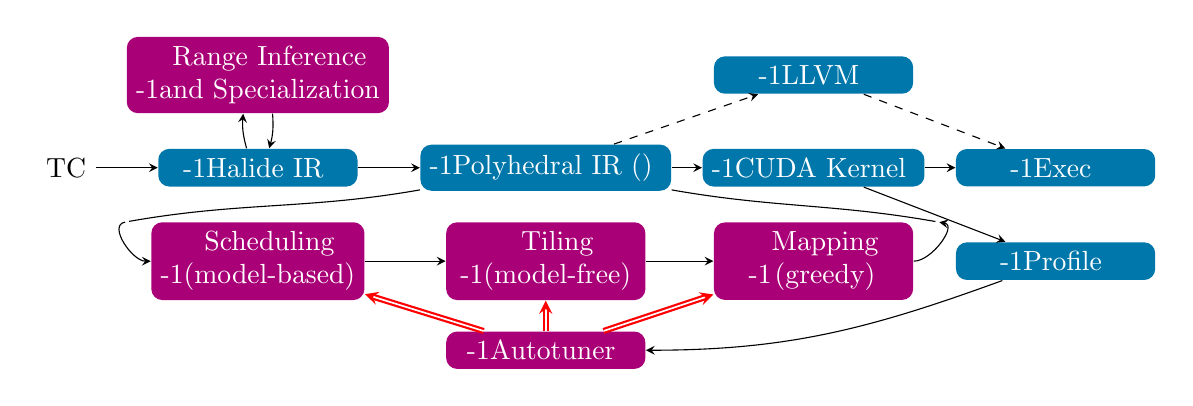
\begin{tikzpicture}[>=stealth]
    \tikzstyle{WIP} = [dashed]
    \tikzstyle{A} = [rectangle, fill=colorA,align=center, text=white,
	font=\relsize{-1},
	minimum width=7.2em, text centered, rounded corners,
	minimum height=1.2em]
    \tikzstyle{B} = [rectangle, fill=colorB,align=center, text=white,
	font=\relsize{-1},
	minimum width=7.2em, text centered, rounded corners,
	minimum height=1.2em]
    \tikzstyle{tune} = [draw,double,->,red,thick]
    \matrix[row sep=0.4cm,column sep=0.4cm,ampersand replacement=\&] {
    \&
    \node[B] (inference) { Range Inference \\ and Specialization };
    \&
    \& \node[A] (LLVM) { LLVM };
    \\
    \node (TC) {TC};
    \&
    \node[A] (Halide) { Halide IR };
    \& \node[A] (isl) { Polyhedral IR (\isl) };
    \& \node[A] (kernel) { CUDA Kernel };
    \& \node[A] (exec) { Exec };
    \\
    \& \node[B] (scheduling) { Scheduling \\ (model-based) };
    \& \node[B] (tiling) { Tiling \\ (model-free) };
    \& \node[B] (mapping) { Mapping \\ (greedy) };
    \& \node[A] (profile) { Profile };
    \\
    \&
    \& \node[B] (autotuner) { Autotuner };
    \\
    };
    \path[draw,->] (TC) -- (Halide);
    \path[draw,->] (Halide) -- (isl);
    \path[draw,->,bend left=10,transform canvas={xshift=-1mm}] (Halide) to (inference);
    \path[draw,->,bend left=10,transform canvas={xshift=1mm}] (inference) to (Halide);
    \node[xshift=-0.3cm,inner sep=0pt] (left) at (scheduling.north west) {};
    \path[draw,->] (isl) to [out=-170,in=10] (left)
			to [out=-170,in=-180] (scheduling);
    \node[xshift=0.3cm,inner sep=0pt] (right) at (mapping.north east) {};
    \path[draw,<-] (isl) to [out=-10,in=170] (right)
			to [out=-10,in=0] (mapping);
    \path[draw,->] (scheduling) -- (tiling);
    \path[draw,->] (tiling) -- (mapping);
    \path[draw,->,WIP] (isl) -- (LLVM);
    \path[draw,->] (isl) -- (kernel);
    \path[draw,->] (kernel) -- (exec);
    \path[draw,->,WIP] (LLVM) -- (exec);
    \path[draw,->] (kernel) -- (profile);
    \path[draw,->] (profile) to[out=-160,in=0] (autotuner);
    \path[tune] (autotuner) -- (scheduling);
    \path[tune] (autotuner) -- (tiling);
    \path[tune] (autotuner) -- (mapping);
    \end{tikzpicture}
}
    \end{minipage}
    \vskip-1ex
  \caption{The JIT compilation flow lowers TC to Halide-IR, then to Polyhedral-IR, followed by optimization, code generation and execution}
  \label{fig:flow}
\end{figure}

The Tensor Comprehensions workflow consists of several stages, progressively
lowering the level of abstraction (Figure~\ref{fig:flow}).
Given a TC with specialized tensor sizes and strides,\footnote{Our
  toolchain supports parametric specifications, yet we have found
  early specialization to be beneficial in driving profitability
  decisions during polyhedral scheduling.} we lower it to a parametric
Halide-IR expression, which is further lowered to a polyhedral
representation where most transformations are applied.  The output of the
polyhedral flow is CUDA code that can be further JIT-compiled with NVRTC and
executed.  Complementing this flow, an autotuner and serializable compilation
engine interacts with scheduling and mapping strategies to search the
optimization space.

Much of TC's versatility and effectiveness resides in its embedding of a
polyhedral compiler as the main optimization engine. The polyhedral framework
is an algebraic representation of ``sufficiently regular'' program parts,
covering arithmetic expressions on arrays surrounded by static control
flow~\cite{Feautrier2011Polyhedron}.  It has been a cornerstone of loop
optimization in the last three
decades~\cite{Irigoin1988Supernode,feautrier92multi,Ancourt1991Scanning,Bastoul2004CLooG,Bondhugula2008Pluto,PPCG2013}
and is integrated into production
compilers~\cite{Trifunovic2010graphite,RStream,Grosser2012Polly,IBMXL}.
Despite its deceiving apparent simplicity, it covers a large class of
computationally-intensive kernels. It is parametric on loop bounds and array
sizes, and captures more transformations of the control and data flow
than domain-specific representations such as
Halide~\cite{Halide} or TVM~\cite{TVM}.  The use of the polyhedral model by
\ourtoolkitname is derived from that of \ppcg~\cite{PPCG2013} and this section
only provides a general overview.
Our transformation engine comprises the following, specially adapted or
algorithmically novel components:
\begin{enumerate}
\item range inference and lowering from high-level TC abstraction to the
  polyhedral representation;
\item core affine scheduling adapted from \isl\ which
  automatically optimizes for (outer) loop parallelism and locality, 
  tuned towards folding a complete TC function into a single GPU kernel;
\item the schedule is further tiled to facilitate the mapping and
  temporal reuse on the deep parallelism and memory hierarchy of
  GPUs~\cite{Verdoolaege2017scheduler};
\item mapping to GPUs borrows from \ppcg~\cite{PPCG2013} with
  extensions to support the more complex and imperfectly
  nested control structures of ML kernels;
\item memory promotion deals with explicit data transfers to and from
  shared and private memory.
\end{enumerate}

\noindent
\emph{This work demonstrates that the polyhedral framework is particularly
  well suited for deep neural networks, featuring large and deeply
  nested loops with long dependence chains and non-uniform or all-to-all
  patterns---arising from fully connected layers and tensor contractions, and
  transpositions. These features push the optimization problem into a
  different heuristic space than Halide's for image processing, and a
  wider space than linear algebra alone.}

\subsection{Range Inference}\label{sec:range_inference}
TC loops are implicit and output tensor sizes are inferred from index
ranges, which themselves may also be inferred.  Our algorithm infers the
largest rectangular ranges that avoid out-of-bounds reads on inputs.
A \ic{where} clause allows for disambiguation if multiple such ranges exist.

Consider the \ic{conv2d} kernel on page~\pageref{page:conv2d}.  The sizes of
the input tensors, \ic{in} and \ic{weight}, are known from the function
signature.  The algorithm needs to infer the ranges of the iterators, and the
size of the output tensor \ic{out}.  The iterators \ic{b}, \ic{op}, \ic{kh},
\ic{kw} appear only once on the RHS and their ranges are therefore $[0, \ic{B})$,
$[0, \ic{OP})$, $[0, \ic{KH})$, $[0, \ic{KW})$ so that they index the input tensors
maximally.  The iterator \ic{ip} appears twice, but indexes the dimension of
the same size, so its range is $[0, \ic{IP})$.
Had it been indexing dimensions of
different sizes, its range would have been the intersection of all size-imposed
ranges.  Once the ranges of \ic{kh} and \ic{kw} are known, it is possible to
infer those of \ic{h} and \ic{w}: we require $\ic{h} + \ic{kh} \leq \ic{H}$ and $\ic{w} + \ic{kw} \leq \ic{W}$,
which leads to the maximal ranges of $[0, \ic{H} - \ic{KH})$ and $[0, \ic{W} - \ic{KW})$
respectively.  Finally, the size of \ic{out} can be inferred given the ranges
of the iterators that index it, yielding \ic{float(B,OP,H-KW,W-KW)}.  The user of
TC is able to inspect the symbolic sizes inferred for the output tensors using
a command-line flag.

Consider now a typical stencil operation \ic{A(i) += B(i + k) * K(k)}: there are multiple ways to
maximize the ranges of \ic{i} and \ic{k}.  To disambiguate without annotations, range
inference proceeds in rounds.  It maintains a set of index variables whose
ranges are not yet resolved.  Initially, it contains all variables not in any
\ic{where} clause.  Each step considers argument expressions that contain a
single unresolved variable and constructs a boolean condition stating the
accesses are within bounds.  Using Halide~\cite{Halide} mechanisms, range
inference computes the maximal range that satisfies this condition given the
already known ranges of other variables.  If different ranges are computed for
the same variable, they are then intersected.  For the stencil above, in the
first round we ignore the expression \ic{B(i + k)} because it contains multiple
unresolved variables. We use \ic{K(k)} to deduce a range for \ic{k}. In the
second round, \ic{B(i + k)} contains a single unresolved variable, and we use
the already-inferred range of \ic{k} to deduce a maximal range for \ic{i}.
% A formal specification of the range
% inference is left for future work.
